\documentclass[onecolumn,12pt]{article}

\usepackage[left=1in,right=1in,top=1in,bottom=1in]{geometry}

\usepackage{latex8}
\usepackage{epsfig}
\usepackage{url}
\usepackage{fancyhdr}
\usepackage{subfigure}
\usepackage{cite}
\usepackage{xspace}
\usepackage{color}
\usepackage{wrapfig}
\usepackage{multirow}
\usepackage{amsmath}
\usepackage{colortbl}
\usepackage{cancel}
\usepackage{umoline}
\usepackage{setspace}
\usepackage{listings}
\usepackage[ampersand]{easylist}
\usepackage{titling}
\usepackage{tabularx}
\usepackage[table]{xcolor}
\usepackage{tikz}
\usepackage{hyperref}

\usetikzlibrary{shapes.multipart}
\usetikzlibrary{arrows}
\usetikzlibrary{shapes.geometric}
\usetikzlibrary{positioning}
\usetikzlibrary{trees}

\definecolor{lightgray}{rgb}{.9,.9,.9}
\definecolor{darkgray}{rgb}{.4,.4,.4}
\definecolor{purple}{rgb}{0.65, 0.12, 0.82}
\definecolor{deepblue}{rgb}{0,0,0.5}
\definecolor{deepred}{rgb}{0.6,0,0}
\definecolor{deepgreen}{rgb}{0,0.5,0}

\DeclareFixedFont{\ttb}{T1}{txtt}{bx}{n}{12} % for bold
\DeclareFixedFont{\ttm}{T1}{txtt}{m}{n}{12}  % for normal

\setlength{\intextsep}{3pt}
\setlength{\columnsep}{3pt}

% Python style for highlighting
\newcommand\pythonstyle{\lstset{
language=Python,
basicstyle=\ttm,
otherkeywords={self, as},             % Add keywords here
keywordstyle=\ttb\color{deepblue},
emph={MyClass,__init__},          % Custom highlighting
emphstyle=\ttb\color{deepred},    % Custom highlighting style
stringstyle=\color{deepgreen},
frame=tb,                         % Any extra options here
showstringspaces=false            % 
}}

% Python environment
\lstnewenvironment{python}[1][]
{
\pythonstyle
\lstset{#1}
}
{}
% Python for inline
\newcommand\pythoninline[1]{{\pythonstyle\lstinline!#1!}}

\lstdefinelanguage{JavaScript}{
  keywords={typeof, new, true, false, catch, function, return, null, catch, switch, var, if, in, while, do, else, case, break},
  keywordstyle=\color{blue}\bfseries,
  ndkeywords={class, export, boolean, throw, implements, import, this},
  ndkeywordstyle=\color{darkgray}\bfseries,
  identifierstyle=\color{black},
  sensitive=false,
  comment=[l]{//},
  morecomment=[s]{/*}{*/},
  commentstyle=\color{purple}\ttfamily,
  stringstyle=\color{red}\ttfamily,
  morestring=[b]',
  morestring=[b]"
}

\usetikzlibrary{arrows,positioning} 
\tikzset{
    %Define standard arrow tip
    >=stealth',
    %Define style for boxes
    box/.style={
           rectangle,
           rounded corners,
           draw=black, very thick,
           minimum height=2em,
           text centered},
    % Define arrow style
    arrow/.style={
           <->,
           thick,
           %shorten <=2pt,
           %shorten >=2pt,
					}
}

\begin{document}


The primary thrust of my work is about Big Data Science as a context for introductory programming, but in order to use this as the context, it must be facilitated through certain new technologies.
I've already had preliminary success in providing data sources through python libraries with a caching layer, but this is only part of the problem that beginners have during their introductory learning experience.
It is unreasonable to expect that a novel context alone will have meaningful impact on students learning experience -- the context does not live in a vacuum, but is part of a system with complex interactions.
The context is a crucial part of a students introductory learning experience, but I think it will prove unfruitful to study it in isolation from other components; therefore, I'm positing my existing research in the broader problem of ``introductory computing experiences''.
The proposed experience for a learner has a context of Big Data Science, facilitated through a Block-based Programming Environment that's tuned for Big Data Science exploration.

This Block-based programming environment (named ``Kennel'' for now) features high-level support for my data sources.
I direct your attention to figure \ref{fig-kennel}, which demonstrates the current version of Kennel that has been used in the Computational Thinking course.
You can see the integration of the data sources through the Data blocks in the lower left.

Using these data sources becomes relatively trivial, and adds important motivation to the context.
However, this in and of itself is insufficient for getting students to succeed.
Think of my existing work as half the battle, the part where we get students to want to succeed (and indeed, I have survey data that suggests that we have motivated students); now we need to be able to guide them to actually succeed.
Success in this case is defined as the students creating algorithmic solutions to computational problems (whether self-directed or after being given a problem) in a serious programming environment such as Spyder, Eclipse, PyCharm, etc..
In order to get them there, I'm proposing several pieces of technology that build on the state-of-the-art.
Although this may seem diverged from what I've been doing before, it's all part of a slightly bigger picture of getting introductory students to success.
I've proven that this context motivates them - now I need to show that, given the right facilitations, instructors can use to motivate them and get them to perform to some specified level of performance.
So, what is this block-based environment that I want to build?

First, let me stop referring to it as the block-based programming environment, and instead refer to it as a Data Science Environment for beginners.
It has a large amount of technology wrapped up in it, and the Block-based component is the least interesting from a research perspective (the Snap! people have already proven that BBP is effective).
So let me make a list of the different technologies and why they are crucial to it:
\begin{description}
  \item[Big Data Sources] This is most important component -- the same libraries that work in Python/Java/Racket need to work in this environment, to really make it so students can explore a useful and empowered context. I'll be leveraging Jonathon's technology to make it so that users can connect to arbitrary data sources, but there'll also be a lot of built-in ones. The same caching mechanisms and lessons that I've learned from my existing work all apply to this.
	\item[Browser-based] This environment needs to be readily available to instructors, with no trips to the server that are unnecessary. I've sewn together Blockly and Skulpt to do this heavy lifting -- everything happens quickly on the client, and we aren't tied to a single LMS.
	\item[Visualization] You can't really do much with data if you're not visualizing it -- seriously, you can only calculate the average temperature in a city so many times before it gets old. By having rich visualizations, you open a whole other dimension of problems. This is part of my research's ongoing conversation about ``what kinds of problems and questions can we ask students using Big Data Science?''
  \item[Big Data Exploration] Students struggle with getting to know the data, and there are things that the interface will be able to do -- Spyder (a Python programming environment) is able to break down the current value of complex variables after code is run, in a series of nested windows (e.g., a list of dictionaries of integer values can be shown in multiple windows). This kind of visualization can be explored to see how it support students' understanding.
	\item[Mutual-Language Transformation] \cite{Matsuzawa} published a paper on this at SIGCSE this year, and its one of the more interesting technical problems. The goal is to get students to be writing code in a real environment, not connecting blocks. I can show data from the Computational Thinking class that shows that students \textit{want} to outgrow the blocks and start doing real-stuff (not all students, but a good number). MLT lets them get to that point in a seamless way. At the same time, we had many students unaware of how to take advantage of this, so there's a lot of research potential in figuring out how to get students to use it gracefully. And from the systems side, its actually really hard to create a semantic block-based mapping to text for a dynamic programming language like Python - tons of interesting little technical challenges. I already have a working version of this.
	\item[Inline Code Blocks] \cite{Weintrop} presented a poster in the SRC on this at SIGCSE this year, and its also very interesting. Much like the MLT, this is meant to let students transition to writing real code. It may be more effective -- it's an open-ended problem.
	\item[Problem Support] Students make a lot of mistakes, and most of these can be picked up automatically -- for example, not knowing to use iteration, or trying to iterate over an empty list. Human instructors are in short demand, so this environment should be able to provide some level of guidance that can help alleviate the bigger mistakes that students have with a given question. This is a mixture of static and dynamic program analysis.
	\item[Student Tracking] The system needs to be able to keep track of all the students and stuff, so the staff can know who's struggling. This means logging student work.
\end{description}

Most of these things are technical features, but they all support the overarching research question of how we can motivate and guide students to explore Computing via Big Data Science - they're facilitations.
I don't think I can do much interesting work without doing them.
Now, they may not all feature in my prelim, but I think it's a convincing story to fit them all together into the same environment in order to guide students.
A big question is how to know what is helping and what isn't -- the answer is user studies, log analysis, surveys, and instructor reports.
That'll be how I collect data on the different components.

\begin{figure}
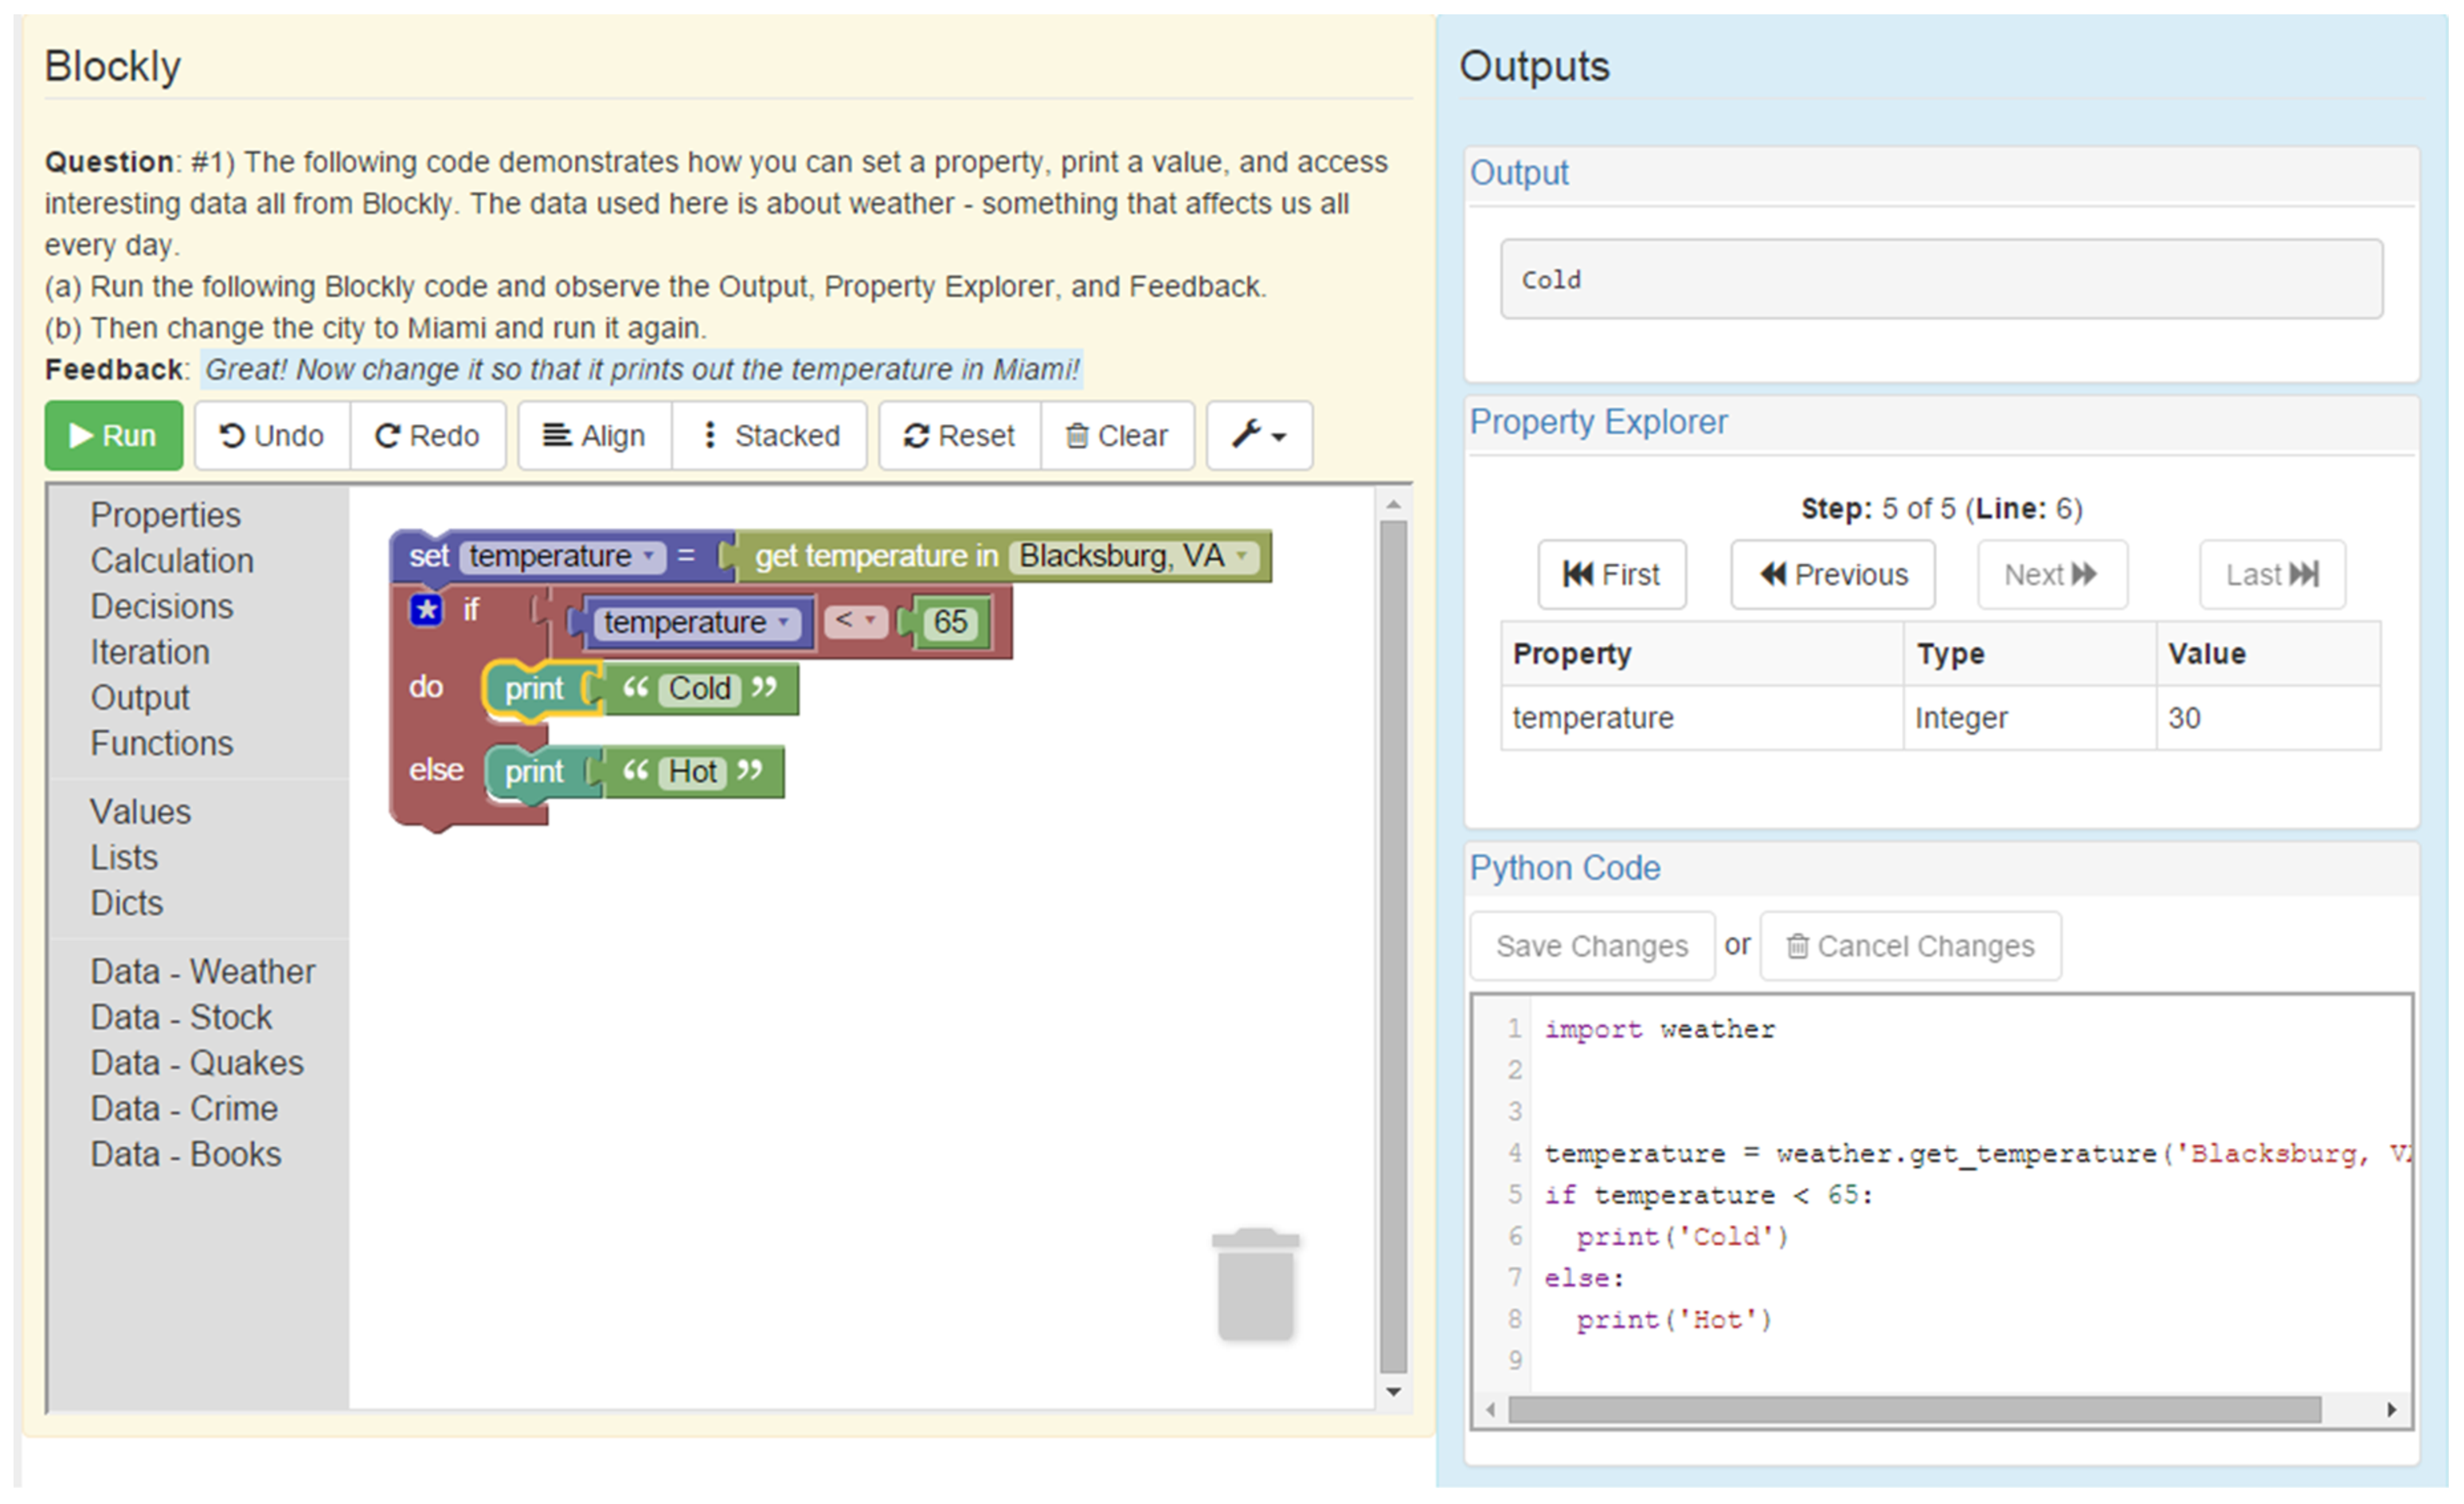
\psfig{file=images/full-kennel.eps, width=\linewidth}
\caption{Current Version of Kennel}
\label{fig-kennel}
\end{figure}

    \bibliographystyle{abbrv}
    
    \bibliography{references}
        
\end{document}